\documentclass{report}
\usepackage{nicematrix,tikz}
\usetikzlibrary{arrows.meta,
                matrix,
                quotes}

%%%%%%%%%%%%%%%%%%%%%%%%%%%%%%%%%
% PACKAGE IMPORTS
%%%%%%%%%%%%%%%%%%%%%%%%%%%%%%%%%


\usepackage[tmargin=2cm,rmargin=1in,lmargin=1in,margin=0.85in,bmargin=2cm,footskip=.2in]{geometry}
\usepackage{amsmath,amsfonts,amsthm,amssymb,mathtools}
\usepackage[varbb]{newpxmath}
\usepackage{xfrac}
\usepackage[makeroom]{cancel}
\usepackage{mathtools}
\usepackage{bookmark}
\usepackage{enumitem}
\usepackage{hyperref,theoremref}
\hypersetup{
	pdftitle={Assignment},
	colorlinks=true, linkcolor=doc!90,
	bookmarksnumbered=true,
	bookmarksopen=true
}
\usepackage[most,many,breakable]{tcolorbox}
\usepackage{xcolor}
\usepackage{varwidth}
\usepackage{varwidth}
\usepackage{etoolbox}
%\usepackage{authblk}
\usepackage{nameref}
\usepackage{multicol,array}
\usepackage{tikz-cd}
\usepackage[ruled,vlined,linesnumbered]{algorithm2e}
\usepackage{comment} % enables the use of multi-line comments (\ifx \fi) 
\usepackage{import}
\usepackage{xifthen}
\usepackage{pdfpages}
\usepackage{transparent}

\newcommand\mycommfont[1]{\footnotesize\ttfamily\textcolor{blue}{#1}}
\SetCommentSty{mycommfont}
\newcommand{\incfig}[1]{%
    \def\svgwidth{\columnwidth}
    \import{./figures/}{#1.pdf_tex}
}

\usepackage{tikzsymbols}
\renewcommand\qedsymbol{$\Laughey$}


%\usepackage{import}
%\usepackage{xifthen}
%\usepackage{pdfpages}
%\usepackage{transparent}


%%%%%%%%%%%%%%%%%%%%%%%%%%%%%%
% SELF MADE COLORS
%%%%%%%%%%%%%%%%%%%%%%%%%%%%%%



\definecolor{myg}{RGB}{56, 140, 70}
\definecolor{myb}{RGB}{45, 111, 177}
\definecolor{myr}{RGB}{199, 68, 64}
\definecolor{mytheorembg}{HTML}{F2F2F9}
\definecolor{mytheoremfr}{HTML}{00007B}
\definecolor{mylenmabg}{HTML}{FFFAF8}
\definecolor{mylenmafr}{HTML}{983b0f}
\definecolor{mypropbg}{HTML}{f2fbfc}
\definecolor{mypropfr}{HTML}{191971}
\definecolor{myexamplebg}{HTML}{F2FBF8}
\definecolor{myexamplefr}{HTML}{88D6D1}
\definecolor{myexampleti}{HTML}{2A7F7F}
\definecolor{mydefinitbg}{HTML}{E5E5FF}
\definecolor{mydefinitfr}{HTML}{3F3FA3}
\definecolor{notesgreen}{RGB}{0,162,0}
\definecolor{myp}{RGB}{197, 92, 212}
\definecolor{mygr}{HTML}{2C3338}
\definecolor{myred}{RGB}{127,0,0}
\definecolor{myyellow}{RGB}{169,121,69}
\definecolor{myexercisebg}{HTML}{F2FBF8}
\definecolor{myexercisefg}{HTML}{88D6D1}


%%%%%%%%%%%%%%%%%%%%%%%%%%%%
% TCOLORBOX SETUPS
%%%%%%%%%%%%%%%%%%%%%%%%%%%%

\setlength{\parindent}{1cm}
%================================
% THEOREM BOX
%================================

\tcbuselibrary{theorems,skins,hooks}
\newtcbtheorem[number within=section]{Theorem}{Theorem}
{%
	enhanced,
	breakable,
	colback = mytheorembg,
	frame hidden,
	boxrule = 0sp,
	borderline west = {2pt}{0pt}{mytheoremfr},
	sharp corners,
	detach title,
	before upper = \tcbtitle\par\smallskip,
	coltitle = mytheoremfr,
	fonttitle = \bfseries\sffamily,
	description font = \mdseries,
	separator sign none,
	segmentation style={solid, mytheoremfr},
}
{th}

\tcbuselibrary{theorems,skins,hooks}
\newtcbtheorem[number within=chapter]{theorem}{Theorem}
{%
	enhanced,
	breakable,
	colback = mytheorembg,
	frame hidden,
	boxrule = 0sp,
	borderline west = {2pt}{0pt}{mytheoremfr},
	sharp corners,
	detach title,
	before upper = \tcbtitle\par\smallskip,
	coltitle = mytheoremfr,
	fonttitle = \bfseries\sffamily,
	description font = \mdseries,
	separator sign none,
	segmentation style={solid, mytheoremfr},
}
{th}


\tcbuselibrary{theorems,skins,hooks}
\newtcolorbox{Theoremcon}
{%
	enhanced
	,breakable
	,colback = mytheorembg
	,frame hidden
	,boxrule = 0sp
	,borderline west = {2pt}{0pt}{mytheoremfr}
	,sharp corners
	,description font = \mdseries
	,separator sign none
}

%================================
% Corollery
%================================
\tcbuselibrary{theorems,skins,hooks}
\newtcbtheorem[number within=section]{Corollary}{Corollary}
{%
	enhanced
	,breakable
	,colback = myp!10
	,frame hidden
	,boxrule = 0sp
	,borderline west = {2pt}{0pt}{myp!85!black}
	,sharp corners
	,detach title
	,before upper = \tcbtitle\par\smallskip
	,coltitle = myp!85!black
	,fonttitle = \bfseries\sffamily
	,description font = \mdseries
	,separator sign none
	,segmentation style={solid, myp!85!black}
}
{th}
\tcbuselibrary{theorems,skins,hooks}
\newtcbtheorem[number within=chapter]{corollary}{Corollary}
{%
	enhanced
	,breakable
	,colback = myp!10
	,frame hidden
	,boxrule = 0sp
	,borderline west = {2pt}{0pt}{myp!85!black}
	,sharp corners
	,detach title
	,before upper = \tcbtitle\par\smallskip
	,coltitle = myp!85!black
	,fonttitle = \bfseries\sffamily
	,description font = \mdseries
	,separator sign none
	,segmentation style={solid, myp!85!black}
}
{th}


%================================
% LENMA
%================================

\tcbuselibrary{theorems,skins,hooks}
\newtcbtheorem[number within=section]{Lenma}{Lenma}
{%
	enhanced,
	breakable,
	colback = mylenmabg,
	frame hidden,
	boxrule = 0sp,
	borderline west = {2pt}{0pt}{mylenmafr},
	sharp corners,
	detach title,
	before upper = \tcbtitle\par\smallskip,
	coltitle = mylenmafr,
	fonttitle = \bfseries\sffamily,
	description font = \mdseries,
	separator sign none,
	segmentation style={solid, mylenmafr},
}
{th}

\tcbuselibrary{theorems,skins,hooks}
\newtcbtheorem[number within=chapter]{lenma}{Lenma}
{%
	enhanced,
	breakable,
	colback = mylenmabg,
	frame hidden,
	boxrule = 0sp,
	borderline west = {2pt}{0pt}{mylenmafr},
	sharp corners,
	detach title,
	before upper = \tcbtitle\par\smallskip,
	coltitle = mylenmafr,
	fonttitle = \bfseries\sffamily,
	description font = \mdseries,
	separator sign none,
	segmentation style={solid, mylenmafr},
}
{th}


%================================
% PROPOSITION
%================================

\tcbuselibrary{theorems,skins,hooks}
\newtcbtheorem[number within=section]{Prop}{Proposition}
{%
	enhanced,
	breakable,
	colback = mypropbg,
	frame hidden,
	boxrule = 0sp,
	borderline west = {2pt}{0pt}{mypropfr},
	sharp corners,
	detach title,
	before upper = \tcbtitle\par\smallskip,
	coltitle = mypropfr,
	fonttitle = \bfseries\sffamily,
	description font = \mdseries,
	separator sign none,
	segmentation style={solid, mypropfr},
}
{th}

\tcbuselibrary{theorems,skins,hooks}
\newtcbtheorem[number within=chapter]{prop}{Proposition}
{%
	enhanced,
	breakable,
	colback = mypropbg,
	frame hidden,
	boxrule = 0sp,
	borderline west = {2pt}{0pt}{mypropfr},
	sharp corners,
	detach title,
	before upper = \tcbtitle\par\smallskip,
	coltitle = mypropfr,
	fonttitle = \bfseries\sffamily,
	description font = \mdseries,
	separator sign none,
	segmentation style={solid, mypropfr},
}
{th}


%================================
% CLAIM
%================================

\tcbuselibrary{theorems,skins,hooks}
\newtcbtheorem[number within=section]{claim}{Claim}
{%
	enhanced
	,breakable
	,colback = myg!10
	,frame hidden
	,boxrule = 0sp
	,borderline west = {2pt}{0pt}{myg}
	,sharp corners
	,detach title
	,before upper = \tcbtitle\par\smallskip
	,coltitle = myg!85!black
	,fonttitle = \bfseries\sffamily
	,description font = \mdseries
	,separator sign none
	,segmentation style={solid, myg!85!black}
}
{th}



%================================
% Exercise
%================================

\tcbuselibrary{theorems,skins,hooks}
\newtcbtheorem[number within=section]{Exercise}{Exercise}
{%
	enhanced,
	breakable,
	colback = myexercisebg,
	frame hidden,
	boxrule = 0sp,
	borderline west = {2pt}{0pt}{myexercisefg},
	sharp corners,
	detach title,
	before upper = \tcbtitle\par\smallskip,
	coltitle = myexercisefg,
	fonttitle = \bfseries\sffamily,
	description font = \mdseries,
	separator sign none,
	segmentation style={solid, myexercisefg},
}
{th}

\tcbuselibrary{theorems,skins,hooks}
\newtcbtheorem[number within=chapter]{exercise}{Exercise}
{%
	enhanced,
	breakable,
	colback = myexercisebg,
	frame hidden,
	boxrule = 0sp,
	borderline west = {2pt}{0pt}{myexercisefg},
	sharp corners,
	detach title,
	before upper = \tcbtitle\par\smallskip,
	coltitle = myexercisefg,
	fonttitle = \bfseries\sffamily,
	description font = \mdseries,
	separator sign none,
	segmentation style={solid, myexercisefg},
}
{th}

%================================
% EXAMPLE BOX
%================================

\newtcbtheorem[number within=section]{Example}{Example}
{%
	colback = myexamplebg
	,breakable
	,colframe = myexamplefr
	,coltitle = myexampleti
	,boxrule = 1pt
	,sharp corners
	,detach title
	,before upper=\tcbtitle\par\smallskip
	,fonttitle = \bfseries
	,description font = \mdseries
	,separator sign none
	,description delimiters parenthesis
}
{ex}

\newtcbtheorem[number within=chapter]{example}{Example}
{%
	colback = myexamplebg
	,breakable
	,colframe = myexamplefr
	,coltitle = myexampleti
	,boxrule = 1pt
	,sharp corners
	,detach title
	,before upper=\tcbtitle\par\smallskip
	,fonttitle = \bfseries
	,description font = \mdseries
	,separator sign none
	,description delimiters parenthesis
}
{ex}

%================================
% DEFINITION BOX
%================================

\newtcbtheorem[number within=section]{Definition}{Definition}{enhanced,
	before skip=2mm,after skip=2mm, colback=red!5,colframe=red!80!black,boxrule=0.5mm,
	attach boxed title to top left={xshift=1cm,yshift*=1mm-\tcboxedtitleheight}, varwidth boxed title*=-3cm,
	boxed title style={frame code={
					\path[fill=tcbcolback]
					([yshift=-1mm,xshift=-1mm]frame.north west)
					arc[start angle=0,end angle=180,radius=1mm]
					([yshift=-1mm,xshift=1mm]frame.north east)
					arc[start angle=180,end angle=0,radius=1mm];
					\path[left color=tcbcolback!60!black,right color=tcbcolback!60!black,
						middle color=tcbcolback!80!black]
					([xshift=-2mm]frame.north west) -- ([xshift=2mm]frame.north east)
					[rounded corners=1mm]-- ([xshift=1mm,yshift=-1mm]frame.north east)
					-- (frame.south east) -- (frame.south west)
					-- ([xshift=-1mm,yshift=-1mm]frame.north west)
					[sharp corners]-- cycle;
				},interior engine=empty,
		},
	fonttitle=\bfseries,
	title={#2},#1}{def}
\newtcbtheorem[number within=chapter]{definition}{Definition}{enhanced,
	before skip=2mm,after skip=2mm, colback=red!5,colframe=red!80!black,boxrule=0.5mm,
	attach boxed title to top left={xshift=1cm,yshift*=1mm-\tcboxedtitleheight}, varwidth boxed title*=-3cm,
	boxed title style={frame code={
					\path[fill=tcbcolback]
					([yshift=-1mm,xshift=-1mm]frame.north west)
					arc[start angle=0,end angle=180,radius=1mm]
					([yshift=-1mm,xshift=1mm]frame.north east)
					arc[start angle=180,end angle=0,radius=1mm];
					\path[left color=tcbcolback!60!black,right color=tcbcolback!60!black,
						middle color=tcbcolback!80!black]
					([xshift=-2mm]frame.north west) -- ([xshift=2mm]frame.north east)
					[rounded corners=1mm]-- ([xshift=1mm,yshift=-1mm]frame.north east)
					-- (frame.south east) -- (frame.south west)
					-- ([xshift=-1mm,yshift=-1mm]frame.north west)
					[sharp corners]-- cycle;
				},interior engine=empty,
		},
	fonttitle=\bfseries,
	title={#2},#1}{def}



%================================
% Solution BOX
%================================

\makeatletter
\newtcbtheorem{question}{Question}{enhanced,
	breakable,
	colback=white,
	colframe=myb!80!black,
	attach boxed title to top left={yshift*=-\tcboxedtitleheight},
	fonttitle=\bfseries,
	title={#2},
	boxed title size=title,
	boxed title style={%
			sharp corners,
			rounded corners=northwest,
			colback=tcbcolframe,
			boxrule=0pt,
		},
	underlay boxed title={%
			\path[fill=tcbcolframe] (title.south west)--(title.south east)
			to[out=0, in=180] ([xshift=5mm]title.east)--
			(title.center-|frame.east)
			[rounded corners=\kvtcb@arc] |-
			(frame.north) -| cycle;
		},
	#1
}{def}
\makeatother

%================================
% SOLUTION BOX
%================================

\makeatletter
\newtcolorbox{solution}{enhanced,
	breakable,
	colback=white,
	colframe=myg!80!black,
	attach boxed title to top left={yshift*=-\tcboxedtitleheight},
	title=Solution,
	boxed title size=title,
	boxed title style={%
			sharp corners,
			rounded corners=northwest,
			colback=tcbcolframe,
			boxrule=0pt,
		},
	underlay boxed title={%
			\path[fill=tcbcolframe] (title.south west)--(title.south east)
			to[out=0, in=180] ([xshift=5mm]title.east)--
			(title.center-|frame.east)
			[rounded corners=\kvtcb@arc] |-
			(frame.north) -| cycle;
		},
}
\makeatother

%================================
% Question BOX
%================================

\makeatletter
\newtcbtheorem{qstion}{Question}{enhanced,
	breakable,
	colback=white,
	colframe=mygr,
	attach boxed title to top left={yshift*=-\tcboxedtitleheight},
	fonttitle=\bfseries,
	title={#2},
	boxed title size=title,
	boxed title style={%
			sharp corners,
			rounded corners=northwest,
			colback=tcbcolframe,
			boxrule=0pt,
		},
	underlay boxed title={%
			\path[fill=tcbcolframe] (title.south west)--(title.south east)
			to[out=0, in=180] ([xshift=5mm]title.east)--
			(title.center-|frame.east)
			[rounded corners=\kvtcb@arc] |-
			(frame.north) -| cycle;
		},
	#1
}{def}
\makeatother

\newtcbtheorem[number within=chapter]{wconc}{Wrong Concept}{
	breakable,
	enhanced,
	colback=white,
	colframe=myr,
	arc=0pt,
	outer arc=0pt,
	fonttitle=\bfseries\sffamily\large,
	colbacktitle=myr,
	attach boxed title to top left={},
	boxed title style={
			enhanced,
			skin=enhancedfirst jigsaw,
			arc=3pt,
			bottom=0pt,
			interior style={fill=myr}
		},
	#1
}{def}



%================================
% NOTE BOX
%================================

\usetikzlibrary{arrows,calc,shadows.blur}
\tcbuselibrary{skins}
\newtcolorbox{note}[1][]{%
	enhanced jigsaw,
	colback=gray!20!white,%
	colframe=gray!80!black,
	size=small,
	boxrule=1pt,
	title=\textbf{Note:-},
	halign title=flush center,
	coltitle=black,
	breakable,
	drop shadow=black!50!white,
	attach boxed title to top left={xshift=1cm,yshift=-\tcboxedtitleheight/2,yshifttext=-\tcboxedtitleheight/2},
	minipage boxed title=1.5cm,
	boxed title style={%
			colback=white,
			size=fbox,
			boxrule=1pt,
			boxsep=2pt,
			underlay={%
					\coordinate (dotA) at ($(interior.west) + (-0.5pt,0)$);
					\coordinate (dotB) at ($(interior.east) + (0.5pt,0)$);
					\begin{scope}
						\clip (interior.north west) rectangle ([xshift=3ex]interior.east);
						\filldraw [white, blur shadow={shadow opacity=60, shadow yshift=-.75ex}, rounded corners=2pt] (interior.north west) rectangle (interior.south east);
					\end{scope}
					\begin{scope}[gray!80!black]
						\fill (dotA) circle (2pt);
						\fill (dotB) circle (2pt);
					\end{scope}
				},
		},
	#1,
}

%%%%%%%%%%%%%%%%%%%%%%%%%%%%%%
% SELF MADE COMMANDS
%%%%%%%%%%%%%%%%%%%%%%%%%%%%%%


\newcommand{\thm}[2]{\begin{Theorem}{#1}{}#2\end{Theorem}}
\newcommand{\cor}[2]{\begin{Corollary}{#1}{}#2\end{Corollary}}
\newcommand{\mlenma}[2]{\begin{Lenma}{#1}{}#2\end{Lenma}}
\newcommand{\mprop}[2]{\begin{Prop}{#1}{}#2\end{Prop}}
\newcommand{\clm}[3]{\begin{claim}{#1}{#2}#3\end{claim}}
\newcommand{\wc}[2]{\begin{wconc}{#1}{}\setlength{\parindent}{1cm}#2\end{wconc}}
\newcommand{\thmcon}[1]{\begin{Theoremcon}{#1}\end{Theoremcon}}
\newcommand{\ex}[2]{\begin{Example}{#1}{}#2\end{Example}}
\newcommand{\dfn}[2]{\begin{Definition}[colbacktitle=red!75!black]{#1}{}#2\end{Definition}}
\newcommand{\dfnc}[2]{\begin{definition}[colbacktitle=red!75!black]{#1}{}#2\end{definition}}
\newcommand{\qs}[2]{\begin{question}{#1}{}#2\end{question}}
\newcommand{\pf}[2]{\begin{myproof}[#1]#2\end{myproof}}
\newcommand{\nt}[1]{\begin{note}#1\end{note}}

\newcommand*\circled[1]{\tikz[baseline=(char.base)]{
		\node[shape=circle,draw,inner sep=1pt] (char) {#1};}}
\newcommand\getcurrentref[1]{%
	\ifnumequal{\value{#1}}{0}
	{??}
	{\the\value{#1}}%
}
\newcommand{\getCurrentSectionNumber}{\getcurrentref{section}}
\newenvironment{myproof}[1][\proofname]{%
	\proof[\bfseries #1: ]%
}{\endproof}

\newcommand{\mclm}[2]{\begin{myclaim}[#1]#2\end{myclaim}}
\newenvironment{myclaim}[1][\claimname]{\proof[\bfseries #1: ]}{}

\newcounter{mylabelcounter}

\makeatletter
\newcommand{\setword}[2]{%
	\phantomsection
	#1\def\@currentlabel{\unexpanded{#1}}\label{#2}%
}
\makeatother




\tikzset{
	symbol/.style={
			draw=none,
			every to/.append style={
					edge node={node [sloped, allow upside down, auto=false]{$#1$}}}
		}
}


% deliminators
\DeclarePairedDelimiter{\abs}{\lvert}{\rvert}
\DeclarePairedDelimiter{\norm}{\lVert}{\rVert}

\DeclarePairedDelimiter{\ceil}{\lceil}{\rceil}
\DeclarePairedDelimiter{\floor}{\lfloor}{\rfloor}
\DeclarePairedDelimiter{\round}{\lfloor}{\rceil}

\newsavebox\diffdbox
\newcommand{\slantedromand}{{\mathpalette\makesl{d}}}
\newcommand{\makesl}[2]{%
\begingroup
\sbox{\diffdbox}{$\mathsurround=0pt#1\mathrm{#2}$}%
\pdfsave
\pdfsetmatrix{1 0 0.2 1}%
\rlap{\usebox{\diffdbox}}%
\pdfrestore
\hskip\wd\diffdbox
\endgroup
}
\newcommand{\dd}[1][]{\ensuremath{\mathop{}\!\ifstrempty{#1}{%
\slantedromand\@ifnextchar^{\hspace{0.2ex}}{\hspace{0.1ex}}}%
{\slantedromand\hspace{0.2ex}^{#1}}}}
\ProvideDocumentCommand\dv{o m g}{%
  \ensuremath{%
    \IfValueTF{#3}{%
      \IfNoValueTF{#1}{%
        \frac{\dd #2}{\dd #3}%
      }{%
        \frac{\dd^{#1} #2}{\dd #3^{#1}}%
      }%
    }{%
      \IfNoValueTF{#1}{%
        \frac{\dd}{\dd #2}%
      }{%
        \frac{\dd^{#1}}{\dd #2^{#1}}%
      }%
    }%
  }%
}
\providecommand*{\pdv}[3][]{\frac{\partial^{#1}#2}{\partial#3^{#1}}}
%  - others
\DeclareMathOperator{\Lap}{\mathcal{L}}
\DeclareMathOperator{\Var}{Var} % varience
\DeclareMathOperator{\Cov}{Cov} % covarience
\DeclareMathOperator{\E}{E} % expected

% Since the amsthm package isn't loaded

% I prefer the slanted \leq
\let\oldleq\leq % save them in case they're every wanted
\let\oldgeq\geq
\renewcommand{\leq}{\leqslant}
\renewcommand{\geq}{\geqslant}

% % redefine matrix env to allow for alignment, use r as default
% \renewcommand*\env@matrix[1][r]{\hskip -\arraycolsep
%     \let\@ifnextchar\new@ifnextchar
%     \array{*\c@MaxMatrixCols #1}}


%\usepackage{framed}
%\usepackage{titletoc}
%\usepackage{etoolbox}
%\usepackage{lmodern}


%\patchcmd{\tableofcontents}{\contentsname}{\sffamily\contentsname}{}{}

%\renewenvironment{leftbar}
%{\def\FrameCommand{\hspace{6em}%
%		{\color{myyellow}\vrule width 2pt depth 6pt}\hspace{1em}}%
%	\MakeFramed{\parshape 1 0cm \dimexpr\textwidth-6em\relax\FrameRestore}\vskip2pt%
%}
%{\endMakeFramed}

%\titlecontents{chapter}
%[0em]{\vspace*{2\baselineskip}}
%{\parbox{4.5em}{%
%		\hfill\Huge\sffamily\bfseries\color{myred}\thecontentspage}%
%	\vspace*{-2.3\baselineskip}\leftbar\textsc{\small\chaptername~\thecontentslabel}\\\sffamily}
%{}{\endleftbar}
%\titlecontents{section}
%[8.4em]
%{\sffamily\contentslabel{3em}}{}{}
%{\hspace{0.5em}\nobreak\itshape\color{myred}\contentspage}
%\titlecontents{subsection}
%[8.4em]
%{\sffamily\contentslabel{3em}}{}{}  
%{\hspace{0.5em}\nobreak\itshape\color{myred}\contentspage}



%%%%%%%%%%%%%%%%%%%%%%%%%%%%%%%%%%%%%%%%%%%
% TABLE OF CONTENTS
%%%%%%%%%%%%%%%%%%%%%%%%%%%%%%%%%%%%%%%%%%%

\usepackage{tikz}
\definecolor{doc}{RGB}{0,60,110}
\usepackage{titletoc}
\contentsmargin{0cm}
\titlecontents{chapter}[3.7pc]
{\addvspace{30pt}%
	\begin{tikzpicture}[remember picture, overlay]%
		\draw[fill=doc!60,draw=doc!60] (-7,-.1) rectangle (-0.9,.5);%
		\pgftext[left,x=-3.5cm,y=0.2cm]{\color{white}\Large\sc\bfseries Chapter\ \thecontentslabel};%
	\end{tikzpicture}\color{doc!60}\large\sc\bfseries}%
{}
{}
{\;\titlerule\;\large\sc\bfseries Page \thecontentspage
	\begin{tikzpicture}[remember picture, overlay]
		\draw[fill=doc!60,draw=doc!60] (2pt,0) rectangle (4,0.1pt);
	\end{tikzpicture}}%
\titlecontents{section}[3.7pc]
{\addvspace{2pt}}
{\contentslabel[\thecontentslabel]{2pc}}
{}
{\hfill\small \thecontentspage}
[]
\titlecontents*{subsection}[3.7pc]
{\addvspace{-1pt}\small}
{}
{}
{\ --- \small\thecontentspage}
[ \textbullet\ ][]

\makeatletter
\renewcommand{\tableofcontents}{%
	\chapter*{%
	  \vspace*{-20\p@}%
	  \begin{tikzpicture}[remember picture, overlay]%
		  \pgftext[right,x=15cm,y=0.2cm]{\color{doc!60}\Huge\sc\bfseries \contentsname};%
		  \draw[fill=doc!60,draw=doc!60] (13,-.75) rectangle (20,1);%
		  \clip (13,-.75) rectangle (20,1);
		  \pgftext[right,x=15cm,y=0.2cm]{\color{white}\Huge\sc\bfseries \contentsname};%
	  \end{tikzpicture}}%
	\@starttoc{toc}}
\makeatother


%From M275 "Topology" at SJSU
\newcommand{\id}{\mathrm{id}}
\newcommand{\taking}[1]{\xrightarrow{#1}}
\newcommand{\inv}{^{-1}}

%From M170 "Introduction to Graph Theory" at SJSU
\DeclareMathOperator{\diam}{diam}
\DeclareMathOperator{\ord}{ord}
\newcommand{\defeq}{\overset{\mathrm{def}}{=}}

%From the USAMO .tex files
\newcommand{\ts}{\textsuperscript}
\newcommand{\dg}{^\circ}
\newcommand{\ii}{\item}

% % From Math 55 and Math 145 at Harvard
% \newenvironment{subproof}[1][Proof]{%
% \begin{proof}[#1] \renewcommand{\qedsymbol}{$\blacksquare$}}%
% {\end{proof}}

\newcommand{\liff}{\leftrightarrow}
\newcommand{\lthen}{\rightarrow}
\newcommand{\opname}{\operatorname}
\newcommand{\surjto}{\twoheadrightarrow}
\newcommand{\injto}{\hookrightarrow}
\newcommand{\On}{\mathrm{On}} % ordinals
\DeclareMathOperator{\img}{im} % Image
\DeclareMathOperator{\Img}{Im} % Image
\DeclareMathOperator{\coker}{coker} % Cokernel
\DeclareMathOperator{\Coker}{Coker} % Cokernel
\DeclareMathOperator{\Ker}{Ker} % Kernel
\DeclareMathOperator{\rank}{rank}
\DeclareMathOperator{\Spec}{Spec} % spectrum
\DeclareMathOperator{\Tr}{Tr} % trace
\DeclareMathOperator{\pr}{pr} % projection
\DeclareMathOperator{\ext}{ext} % extension
\DeclareMathOperator{\pred}{pred} % predecessor
\DeclareMathOperator{\dom}{dom} % domain
\DeclareMathOperator{\ran}{ran} % range
\DeclareMathOperator{\Hom}{Hom} % homomorphism
\DeclareMathOperator{\Mor}{Mor} % morphisms
\DeclareMathOperator{\End}{End} % endomorphism

\newcommand{\eps}{\epsilon}
\newcommand{\veps}{\varepsilon}
\newcommand{\ol}{\overline}
\newcommand{\ul}{\underline}
\newcommand{\wt}{\widetilde}
\newcommand{\wh}{\widehat}
\newcommand{\vocab}[1]{\textbf{\color{blue} #1}}
\providecommand{\half}{\frac{1}{2}}
\newcommand{\dang}{\measuredangle} %% Directed angle
\newcommand{\ray}[1]{\overrightarrow{#1}}
\newcommand{\seg}[1]{\overline{#1}}
\newcommand{\arc}[1]{\wideparen{#1}}
\DeclareMathOperator{\cis}{cis}
\DeclareMathOperator*{\lcm}{lcm}
\DeclareMathOperator*{\argmin}{arg min}
\DeclareMathOperator*{\argmax}{arg max}
\newcommand{\cycsum}{\sum_{\mathrm{cyc}}}
\newcommand{\symsum}{\sum_{\mathrm{sym}}}
\newcommand{\cycprod}{\prod_{\mathrm{cyc}}}
\newcommand{\symprod}{\prod_{\mathrm{sym}}}
\newcommand{\Qed}{\begin{flushright}\qed\end{flushright}}
\newcommand{\parinn}{\setlength{\parindent}{1cm}}
\newcommand{\parinf}{\setlength{\parindent}{0cm}}
% \newcommand{\norm}{\|\cdot\|}
\newcommand{\inorm}{\norm_{\infty}}
\newcommand{\opensets}{\{V_{\alpha}\}_{\alpha\in I}}
\newcommand{\oset}{V_{\alpha}}
\newcommand{\opset}[1]{V_{\alpha_{#1}}}
\newcommand{\lub}{\text{lub}}
\newcommand{\del}[2]{\frac{\partial #1}{\partial #2}}
\newcommand{\Del}[3]{\frac{\partial^{#1} #2}{\partial^{#1} #3}}
\newcommand{\deld}[2]{\dfrac{\partial #1}{\partial #2}}
\newcommand{\Deld}[3]{\dfrac{\partial^{#1} #2}{\partial^{#1} #3}}
\newcommand{\lm}{\lambda}
\newcommand{\uin}{\mathbin{\rotatebox[origin=c]{90}{$\in$}}}
\newcommand{\usubset}{\mathbin{\rotatebox[origin=c]{90}{$\subset$}}}
\newcommand{\lt}{\left}
\newcommand{\rt}{\right}
\newcommand{\bs}[1]{\boldsymbol{#1}}
\newcommand{\exs}{\exists}
\newcommand{\st}{\strut}
\newcommand{\dps}[1]{\displaystyle{#1}}

\newcommand{\sol}{\setlength{\parindent}{0cm}\textbf{\textit{Solution:}}\setlength{\parindent}{1cm} }
\newcommand{\solve}[1]{\setlength{\parindent}{0cm}\textbf{\textit{Solution: }}\setlength{\parindent}{1cm}#1 \Qed}

% Things Lie
\newcommand{\kb}{\mathfrak b}
\newcommand{\kg}{\mathfrak g}
\newcommand{\kh}{\mathfrak h}
\newcommand{\kn}{\mathfrak n}
\newcommand{\ku}{\mathfrak u}
\newcommand{\kz}{\mathfrak z}
\DeclareMathOperator{\Ext}{Ext} % Ext functor
\DeclareMathOperator{\Tor}{Tor} % Tor functor
\newcommand{\gl}{\opname{\mathfrak{gl}}} % frak gl group
\renewcommand{\sl}{\opname{\mathfrak{sl}}} % frak sl group chktex 6

% More script letters etc.
\newcommand{\SA}{\mathcal A}
\newcommand{\SB}{\mathcal B}
\newcommand{\SC}{\mathcal C}
\newcommand{\SF}{\mathcal F}
\newcommand{\SG}{\mathcal G}
\newcommand{\SH}{\mathcal H}
\newcommand{\OO}{\mathcal O}

\newcommand{\SCA}{\mathscr A}
\newcommand{\SCB}{\mathscr B}
\newcommand{\SCC}{\mathscr C}
\newcommand{\SCD}{\mathscr D}
\newcommand{\SCE}{\mathscr E}
\newcommand{\SCF}{\mathscr F}
\newcommand{\SCG}{\mathscr G}
\newcommand{\SCH}{\mathscr H}

% Mathfrak primes
\newcommand{\km}{\mathfrak m}
\newcommand{\kp}{\mathfrak p}
\newcommand{\kq}{\mathfrak q}

% number sets
\newcommand{\RR}[1][]{\ensuremath{\ifstrempty{#1}{\mathbb{R}}{\mathbb{R}^{#1}}}}
\newcommand{\NN}[1][]{\ensuremath{\ifstrempty{#1}{\mathbb{N}}{\mathbb{N}^{#1}}}}
\newcommand{\ZZ}[1][]{\ensuremath{\ifstrempty{#1}{\mathbb{Z}}{\mathbb{Z}^{#1}}}}
\newcommand{\QQ}[1][]{\ensuremath{\ifstrempty{#1}{\mathbb{Q}}{\mathbb{Q}^{#1}}}}
\newcommand{\CC}[1][]{\ensuremath{\ifstrempty{#1}{\mathbb{C}}{\mathbb{C}^{#1}}}}
\newcommand{\PP}[1][]{\ensuremath{\ifstrempty{#1}{\mathbb{P}}{\mathbb{P}^{#1}}}}
\newcommand{\HH}[1][]{\ensuremath{\ifstrempty{#1}{\mathbb{H}}{\mathbb{H}^{#1}}}}
\newcommand{\FF}[1][]{\ensuremath{\ifstrempty{#1}{\mathbb{F}}{\mathbb{F}^{#1}}}}
% expected value
\newcommand{\EE}{\ensuremath{\mathbb{E}}}
\newcommand{\charin}{\text{ char }}
\DeclareMathOperator{\sign}{sign}
\DeclareMathOperator{\Aut}{Aut}
\DeclareMathOperator{\Inn}{Inn}
\DeclareMathOperator{\Syl}{Syl}
\DeclareMathOperator{\Gal}{Gal}
\DeclareMathOperator{\GL}{GL} % General linear group
\DeclareMathOperator{\SL}{SL} % Special linear group

%---------------------------------------
% BlackBoard Math Fonts :-
%---------------------------------------

%Captital Letters
\newcommand{\bbA}{\mathbb{A}}	\newcommand{\bbB}{\mathbb{B}}
\newcommand{\bbC}{\mathbb{C}}	\newcommand{\bbD}{\mathbb{D}}
\newcommand{\bbE}{\mathbb{E}}	\newcommand{\bbF}{\mathbb{F}}
\newcommand{\bbG}{\mathbb{G}}	\newcommand{\bbH}{\mathbb{H}}
\newcommand{\bbI}{\mathbb{I}}	\newcommand{\bbJ}{\mathbb{J}}
\newcommand{\bbK}{\mathbb{K}}	\newcommand{\bbL}{\mathbb{L}}
\newcommand{\bbM}{\mathbb{M}}	\newcommand{\bbN}{\mathbb{N}}
\newcommand{\bbO}{\mathbb{O}}	\newcommand{\bbP}{\mathbb{P}}
\newcommand{\bbQ}{\mathbb{Q}}	\newcommand{\bbR}{\mathbb{R}}
\newcommand{\bbS}{\mathbb{S}}	\newcommand{\bbT}{\mathbb{T}}
\newcommand{\bbU}{\mathbb{U}}	\newcommand{\bbV}{\mathbb{V}}
\newcommand{\bbW}{\mathbb{W}}	\newcommand{\bbX}{\mathbb{X}}
\newcommand{\bbY}{\mathbb{Y}}	\newcommand{\bbZ}{\mathbb{Z}}

%---------------------------------------
% MathCal Fonts :-
%---------------------------------------

%Captital Letters
\newcommand{\mcA}{\mathcal{A}}	\newcommand{\mcB}{\mathcal{B}}
\newcommand{\mcC}{\mathcal{C}}	\newcommand{\mcD}{\mathcal{D}}
\newcommand{\mcE}{\mathcal{E}}	\newcommand{\mcF}{\mathcal{F}}
\newcommand{\mcG}{\mathcal{G}}	\newcommand{\mcH}{\mathcal{H}}
\newcommand{\mcI}{\mathcal{I}}	\newcommand{\mcJ}{\mathcal{J}}
\newcommand{\mcK}{\mathcal{K}}	\newcommand{\mcL}{\mathcal{L}}
\newcommand{\mcM}{\mathcal{M}}	\newcommand{\mcN}{\mathcal{N}}
\newcommand{\mcO}{\mathcal{O}}	\newcommand{\mcP}{\mathcal{P}}
\newcommand{\mcQ}{\mathcal{Q}}	\newcommand{\mcR}{\mathcal{R}}
\newcommand{\mcS}{\mathcal{S}}	\newcommand{\mcT}{\mathcal{T}}
\newcommand{\mcU}{\mathcal{U}}	\newcommand{\mcV}{\mathcal{V}}
\newcommand{\mcW}{\mathcal{W}}	\newcommand{\mcX}{\mathcal{X}}
\newcommand{\mcY}{\mathcal{Y}}	\newcommand{\mcZ}{\mathcal{Z}}


%---------------------------------------
% Bold Math Fonts :-
%---------------------------------------

%Captital Letters
\newcommand{\bmA}{\boldsymbol{A}}	\newcommand{\bmB}{\boldsymbol{B}}
\newcommand{\bmC}{\boldsymbol{C}}	\newcommand{\bmD}{\boldsymbol{D}}
\newcommand{\bmE}{\boldsymbol{E}}	\newcommand{\bmF}{\boldsymbol{F}}
\newcommand{\bmG}{\boldsymbol{G}}	\newcommand{\bmH}{\boldsymbol{H}}
\newcommand{\bmI}{\boldsymbol{I}}	\newcommand{\bmJ}{\boldsymbol{J}}
\newcommand{\bmK}{\boldsymbol{K}}	\newcommand{\bmL}{\boldsymbol{L}}
\newcommand{\bmM}{\boldsymbol{M}}	\newcommand{\bmN}{\boldsymbol{N}}
\newcommand{\bmO}{\boldsymbol{O}}	\newcommand{\bmP}{\boldsymbol{P}}
\newcommand{\bmQ}{\boldsymbol{Q}}	\newcommand{\bmR}{\boldsymbol{R}}
\newcommand{\bmS}{\boldsymbol{S}}	\newcommand{\bmT}{\boldsymbol{T}}
\newcommand{\bmU}{\boldsymbol{U}}	\newcommand{\bmV}{\boldsymbol{V}}
\newcommand{\bmW}{\boldsymbol{W}}	\newcommand{\bmX}{\boldsymbol{X}}
\newcommand{\bmY}{\boldsymbol{Y}}	\newcommand{\bmZ}{\boldsymbol{Z}}
%Small Letters
\newcommand{\bma}{\boldsymbol{a}}	\newcommand{\bmb}{\boldsymbol{b}}
\newcommand{\bmc}{\boldsymbol{c}}	\newcommand{\bmd}{\boldsymbol{d}}
\newcommand{\bme}{\boldsymbol{e}}	\newcommand{\bmf}{\boldsymbol{f}}
\newcommand{\bmg}{\boldsymbol{g}}	\newcommand{\bmh}{\boldsymbol{h}}
\newcommand{\bmi}{\boldsymbol{i}}	\newcommand{\bmj}{\boldsymbol{j}}
\newcommand{\bmk}{\boldsymbol{k}}	\newcommand{\bml}{\boldsymbol{l}}
\newcommand{\bmm}{\boldsymbol{m}}	\newcommand{\bmn}{\boldsymbol{n}}
\newcommand{\bmo}{\boldsymbol{o}}	\newcommand{\bmp}{\boldsymbol{p}}
\newcommand{\bmq}{\boldsymbol{q}}	\newcommand{\bmr}{\boldsymbol{r}}
\newcommand{\bms}{\boldsymbol{s}}	\newcommand{\bmt}{\boldsymbol{t}}
\newcommand{\bmu}{\boldsymbol{u}}	\newcommand{\bmv}{\boldsymbol{v}}
\newcommand{\bmw}{\boldsymbol{w}}	\newcommand{\bmx}{\boldsymbol{x}}
\newcommand{\bmy}{\boldsymbol{y}}	\newcommand{\bmz}{\boldsymbol{z}}

%---------------------------------------
% Scr Math Fonts :-
%---------------------------------------

\newcommand{\sA}{{\mathscr{A}}}   \newcommand{\sB}{{\mathscr{B}}}
\newcommand{\sC}{{\mathscr{C}}}   \newcommand{\sD}{{\mathscr{D}}}
\newcommand{\sE}{{\mathscr{E}}}   \newcommand{\sF}{{\mathscr{F}}}
\newcommand{\sG}{{\mathscr{G}}}   \newcommand{\sH}{{\mathscr{H}}}
\newcommand{\sI}{{\mathscr{I}}}   \newcommand{\sJ}{{\mathscr{J}}}
\newcommand{\sK}{{\mathscr{K}}}   \newcommand{\sL}{{\mathscr{L}}}
\newcommand{\sM}{{\mathscr{M}}}   \newcommand{\sN}{{\mathscr{N}}}
\newcommand{\sO}{{\mathscr{O}}}   \newcommand{\sP}{{\mathscr{P}}}
\newcommand{\sQ}{{\mathscr{Q}}}   \newcommand{\sR}{{\mathscr{R}}}
\newcommand{\sS}{{\mathscr{S}}}   \newcommand{\sT}{{\mathscr{T}}}
\newcommand{\sU}{{\mathscr{U}}}   \newcommand{\sV}{{\mathscr{V}}}
\newcommand{\sW}{{\mathscr{W}}}   \newcommand{\sX}{{\mathscr{X}}}
\newcommand{\sY}{{\mathscr{Y}}}   \newcommand{\sZ}{{\mathscr{Z}}}


%---------------------------------------
% Math Fraktur Font
%---------------------------------------

%Captital Letters
\newcommand{\mfA}{\mathfrak{A}}	\newcommand{\mfB}{\mathfrak{B}}
\newcommand{\mfC}{\mathfrak{C}}	\newcommand{\mfD}{\mathfrak{D}}
\newcommand{\mfE}{\mathfrak{E}}	\newcommand{\mfF}{\mathfrak{F}}
\newcommand{\mfG}{\mathfrak{G}}	\newcommand{\mfH}{\mathfrak{H}}
\newcommand{\mfI}{\mathfrak{I}}	\newcommand{\mfJ}{\mathfrak{J}}
\newcommand{\mfK}{\mathfrak{K}}	\newcommand{\mfL}{\mathfrak{L}}
\newcommand{\mfM}{\mathfrak{M}}	\newcommand{\mfN}{\mathfrak{N}}
\newcommand{\mfO}{\mathfrak{O}}	\newcommand{\mfP}{\mathfrak{P}}
\newcommand{\mfQ}{\mathfrak{Q}}	\newcommand{\mfR}{\mathfrak{R}}
\newcommand{\mfS}{\mathfrak{S}}	\newcommand{\mfT}{\mathfrak{T}}
\newcommand{\mfU}{\mathfrak{U}}	\newcommand{\mfV}{\mathfrak{V}}
\newcommand{\mfW}{\mathfrak{W}}	\newcommand{\mfX}{\mathfrak{X}}
\newcommand{\mfY}{\mathfrak{Y}}	\newcommand{\mfZ}{\mathfrak{Z}}
%Small Letters
\newcommand{\mfa}{\mathfrak{a}}	\newcommand{\mfb}{\mathfrak{b}}
\newcommand{\mfc}{\mathfrak{c}}	\newcommand{\mfd}{\mathfrak{d}}
\newcommand{\mfe}{\mathfrak{e}}	\newcommand{\mff}{\mathfrak{f}}
\newcommand{\mfg}{\mathfrak{g}}	\newcommand{\mfh}{\mathfrak{h}}
\newcommand{\mfi}{\mathfrak{i}}	\newcommand{\mfj}{\mathfrak{j}}
\newcommand{\mfk}{\mathfrak{k}}	\newcommand{\mfl}{\mathfrak{l}}
\newcommand{\mfm}{\mathfrak{m}}	\newcommand{\mfn}{\mathfrak{n}}
\newcommand{\mfo}{\mathfrak{o}}	\newcommand{\mfp}{\mathfrak{p}}
\newcommand{\mfq}{\mathfrak{q}}	\newcommand{\mfr}{\mathfrak{r}}
\newcommand{\mfs}{\mathfrak{s}}	\newcommand{\mft}{\mathfrak{t}}
\newcommand{\mfu}{\mathfrak{u}}	\newcommand{\mfv}{\mathfrak{v}}
\newcommand{\mfw}{\mathfrak{w}}	\newcommand{\mfx}{\mathfrak{x}}
\newcommand{\mfy}{\mathfrak{y}}	\newcommand{\mfz}{\mathfrak{z}}


\title{\Huge{Math 2700.009}\\Problem Set 13}
\author{\huge{Ezekiel Berumen}}
\date{23 April 2024}

\begin{document}

\maketitle
\newpage

\qs{}{Consider $C([-\pi, \pi])$ with the inner-product
$$
\langle f \mid g\rangle=\frac{1}{2 \pi} \int_{-\pi}^\pi f(x) g(x) \mathrm{d} x
$$
and $S \subseteq C([-\pi, \pi])$ be
$$
S=\{\sin (n x), \cos (m x): m, n>0\},
$$
verify that $S$ is an orthogonal set in $C([-\pi, \pi])$.}
\begin{note}
Recall:
\begin{itemize}
\item To show a set $S$ is an orthogonal set, we must show that for all $\vec{v},\vec{w}\in S$ the inner-product $\langle \vec{v} \mid \vec{w} \rangle=0$, with $\vec{0}\notin S$
\end{itemize}
\end{note}
\sol Let us begin by finding the inner product $\langle \sin(nx) \mid \cos(mx) \rangle$ when $m \neq n$:
$$
\begin{aligned}
\langle \sin(nx) \mid \cos(mx) \rangle &= \frac{1}{2\pi} \int_{-\pi}^{\pi} \sin(nx)\cos(mx)\mathrm{d}x \\
&= \frac{1}{2\pi} \int_{-\pi}^{\pi} \frac{\sin(nx + mx)+\sin(nx-mx)}{2}\mathrm{d}x\\
&=\frac{1}{4\pi} \left(\int_{-\pi}^{\pi}\sin(nx+mx)\mathrm{d}x + \int_{-\pi}^{\pi}\sin(nx-mx)\mathrm{d}x\right)\\
&=\frac{1}{4\pi} \left(-\frac{1}{n+m}\cos(nx+mx)-\frac{1}{n-m}\cos(nx-mx)\right)\biggr\rvert_{x=-\pi}^\pi\\
&=\begin{aligned}
\frac{1}{4\pi} \left(-\frac{1}{n+m}\right.&\cos(n\pi+m\pi)-\frac{1}{n-m}\cos(n\pi-m\pi) \\
&+\left.\frac{1}{n+m}\cos(n\pi+m\pi)+\frac{1}{n-m}\cos(n\pi-m\pi)\right)
\end{aligned}\\
&=\frac{1}{4\pi}(0)\\
&=0
\end{aligned}
$$
This "proof" only reveals if the vectors are orthogonal in instances where $m\neq n$, so let us review the case where $m = n$ by computing the inner-product $\langle \sin(nx) \mid \cos(nx) \rangle$
$$
\begin{aligned}
\langle \sin(nx) \mid \cos(nx) \rangle &= \frac{1}{2\pi} \int_{-\pi}^{\pi} \sin(nx)\cos(nx)\mathrm{d}x \qquad \left[\begin{aligned}\
\text{Let } u &= \sin(nx)\\
\mathrm{d}u &= \frac{1}{n}\cos(nx)\mathrm{d}x
\end{aligned}\right]\\
&=\frac{1}{2\pi} \int_{-n\pi}^{n\pi} u \frac{\mathrm{d}u}{n} \\
&=\frac{1}{2\pi n} \int_{-n\pi}^{n\pi} u \mathrm{d}u\\
&=\frac{u^2}{4\pi n}\biggr\rvert_{u=-\pi n}^{\pi n}\\
&=\frac{\pi^2 n^2}{4\pi n} - \frac{\pi^2 n^2}{4\pi n}\\
&=0
\end{aligned}
$$
Since we have shown that the inner product $\langle \sin(nx) \mid \cos(mx) \rangle$ is zero regardless of the value of $m$ and $n$, then we can say that $S$ is an orthogonal set.
\qs{}{Let $V$ be an inner-product space with inner-product $\langle\cdot \mid \cdot\rangle$, and $\vec{u}_1, \ldots, \vec{u}_n \in V$. Define a function $T: V \rightarrow V$ by
$$
T(\vec{v})=\sum_{k=1}^n\left\langle\vec{v} \mid \vec{u}_k\right\rangle \vec{u}_k
$$
Verify that $T$ is a linear transformation.}
\begin{note}
Recall that if $T: V \rightarrow V$ is a linear transformation, two properties must be verifiable:
\begin{itemize}
\item Additivity: A function $T: V \rightarrow V$ is additive if for any $\vec{x},\vec{y}\in V$, $T(\vec{x} + \vec{y}) = T(\vec{x}) + T(\vec{y})$
\item Homogeneity: A function $T: V \rightarrow V$ is homogeneous if for any $c\in\mathbb{R}$ and $\vec{x}\in V$, $T(c\vec{x}) = cT(\vec{x})$
\end{itemize}
\end{note}
\sol \\
\begin{itemize}
\item Additivity: Let $\vec{w}\in V$
$$
\begin{aligned}
T(\vec{v} + \vec{w}) &= \sum_{k=1}^n \left\langle\vec{v} + \vec{w} \mid \vec{u}_k\right\rangle \vec{u}_k\\
&=\sum_{k=1}^n \left(\left\langle\vec{v} \mid \vec{u}_k \right\rangle + \left\langle\vec{w} \mid \vec{u}_k\right\rangle\right)\vec{u}_k\\
&=\sum_{k=1}^n \left\langle\vec{v} \mid \vec{u}_k \right\rangle\vec{u}_k + \left\langle\vec{w} \mid \vec{u}_k\right\rangle\vec{u}_k\\
&=\sum_{k=1}^n \left\langle\vec{v} \mid \vec{u}_k \right\rangle\vec{u}_k + \sum_{k=1}^n\left\langle\vec{w} \mid \vec{u}_k\right\rangle\vec{u}_k\\
&=T(\vec{v}) + T(\vec{w})
\end{aligned}
$$
Since $T$ is additive for any $\vec{v},\vec{w}\in V$, then it satisfies the first propery.
\item Homogeneity: Let $c\in\mathbb{R}$
$$
\begin{aligned}
T(c\vec{v}) &= \sum_{k=1}^n \left\langle c\vec{v} \mid \vec{u}_k \right\rangle \vec{u}_k\\
&=\sum_{k=1}^n c\left\langle\vec{v}\mid\vec{u}_k\right\rangle\vec{u}_k\\
&=c\sum_{k=1}^n\left\langle\vec{v}\mid\vec{u}_k\right\rangle\vec{u}_k\\
&=cT(\vec{v})
\end{aligned}
$$
\end{itemize}
Because $T$ is both additive and homogeneous, then it is sufficient to say that it is a linear transformation.
\pagebreak
\qs{}{Let
$$
A=\left[\begin{array}{lll}
1 & 1 & 2 \\
1 & 0 & 1 \\
0 & 2 & 2
\end{array}\right]
$$
(a) Find an ordered basis for $\operatorname{ran}(A)$\\
(b) Perform the Gram-Schmidt algorithm on the basis you got in (a) to get an orthonormal basis for $\operatorname{ran}(A)$\\
(c) Find a basis for $\operatorname{ker}(A)$\\
(d) Extend the basis you found in (a) to a basis $\mathfrak{B}$ for $\mathbb{R}^3$\\
(e) Find $P_{\mathfrak{E} \rightarrow \mathfrak{B} \text {. }}$}
\begin{note}
Recall: \\
\\
\noindent Let $\langle \vec{x}_1, \ldots, \vec{x}_n \rangle$ be a basis for an $n$-dimensional inner-product space $V$. The Gram-Schmidt Algorithm:
$$
\vec{v}_i = \vec{x}_i - \sum_{k=1}^{i-1} \langle \vec{x}_{i} \mid \vec{y}_k \rangle \vec{y}_k, \qquad \vec{y}_i = \vec{v}_i/||\vec{v}_i||
$$
Is used to find an orthogonal basis for $V$ by subtracting all the pieces of $\vec{x}_i$ that are in the same direction as all of the $\vec{y}_k$, then renormalizing. This formula computes normalized vectors that are orthogonal to all other $\vec{y}_k$'s since the non-perpendicular pieces are removed.
\end{note}
\sol \\
(a) We can see that $\vec{a}_1 = \vec{a}_3 - \vec{a}_2$ and thus $\vec{0} = -\vec{a}_1 - \vec{a}_2 + \vec{a}_3$. Since $\vec{a}_1$ is the only linearly dependent vector, then we can say that an ordered basis for the $\ran(A)$ is:
$$
\left\langle 
\begin{bmatrix}1\\0\\2\end{bmatrix},
\begin{bmatrix}2\\1\\2\end{bmatrix}
\right\rangle
$$
(b) We will apply the Gram-Schmidt formula to find the orthonormal basis vectors
$$
\vec{b}_1 = \vec{x}_1 = \begin{bmatrix}1\\0\\2\end{bmatrix}
$$
$$
||\vec{b}_1|| = \sqrt{\vec{b}_1\cdot\vec{b}_1} = \sqrt{1 + 0 + 4} = \sqrt{5} \implies \frac{1}{||\vec{b}_1||} = \frac{1}{\sqrt{5}}
$$
\[
\vec{y}_1 = \frac{1}{\sqrt{5}}\begin{bmatrix}1\\0\\2\end{bmatrix} = \begin{bmatrix} 1/\sqrt{5} \\ 0 \\ 2/\sqrt{5} \end{bmatrix}
\]
\vspace{0.5em}
\hrule
\vspace{1em}
\[
\begin{aligned}
\vec{b}_2 &= \vec{x}_2 - (\vec{y}_1 \cdot \vec{x}_2)\vec{y}_1\\
&=\vec{x}_2 - (2/\sqrt{5} + 0 + 4/\sqrt{5})\vec{y}_1\\
&=\begin{bmatrix}2\\1\\2\end{bmatrix}-6/\sqrt{5}\begin{bmatrix}1\sqrt{5}\\0\\2\sqrt{5}\end{bmatrix}\\
&=\begin{bmatrix}2\\1\\2\end{bmatrix}-\begin{bmatrix}6/5\\0\\12/5\end{bmatrix} = \begin{bmatrix}4/5\\1\\-2/5\end{bmatrix}\\
\end{aligned}
\]
\[
||\vec{b}_2|| = \sqrt{\vec{b}_2\cdot\vec{b}_2} = \sqrt{16/25 + 1 + 4/25} = \sqrt{45/25} = \sqrt{9/5} = 3/\sqrt{5}
\]
\[
\implies \frac{1}{||\vec{b}_2||}=\frac{\sqrt{5}}{3}
\]
\[
\vec{y}_2 = \frac{\sqrt{5}}{3}\begin{bmatrix}4/5\\1\\-2/5\end{bmatrix} = \begin{bmatrix}4\sqrt{5}/15\\\sqrt{5}/3\\-2\sqrt{5}/15\end{bmatrix}
\]
\vspace{0.5em}
\hrule
\vspace{1em}
\noindent The vectors we have found form an orthonormal basis for $\ran(A)$, which is
$$
\left\langle\begin{bmatrix} 1/\sqrt{5} \\ 0 \\ 2/\sqrt{5} \end{bmatrix},\begin{bmatrix}4\sqrt{5}/15\\\sqrt{5}/3\\-2\sqrt{5}/15\end{bmatrix}\right\rangle
$$
(c) To find a basis for the $\ker(A)$, we can use the linearly dependent vector we found in (a). In particular we see that $\vec{0} = -\vec{a}_1 - \vec{a}_2 + \vec{a}_3$. Rank-Nullity tells us that the dimension of the kernel will be one since the dimension of the range is 2. With this information we can say that a basis for $\ker(A)$ is
$$
\left\{\begin{bmatrix}-1\\-1\\1\end{bmatrix}\right\}
$$
(d) We can extend ordered basis we found in (a) to make a basis for $\mathbb{R}^3$ by using the standard basis vector $\vec{e}_3$. We find that
$$
\mathfrak{B} = \left\langle\begin{bmatrix}0\\0\\1\end{bmatrix},\begin{bmatrix}1\\0\\2\end{bmatrix},\begin{bmatrix}2\\1\\2\end{bmatrix}\right\rangle
$$
(e) In order to find $P_{\mathfrak{E}\rightarrow\mathfrak{B}}$ we need to find $P_{\mathfrak{B}\rightarrow\mathfrak{E}}$ and then find its inverse.
$$
P_{\mathfrak{B}\rightarrow\mathfrak{E}} = \begin{bmatrix}0&1&2\\0&0&1\\1&2&2\end{bmatrix}
$$
Now we can find $(P_{\mathfrak{B}\rightarrow\mathfrak{E}})^-1=P_{\mathfrak{E}\rightarrow\mathfrak{B}}$ by using the row reduction method
$$
\begin{aligned}
&\begin{array}{ccc|ccc}
0&1&2&1&0&0\\
0&0&1&0&1&0\\
1&2&2&0&0&1
\end{array}
&& R_1 \leftrightarrow R_3
\qquad
&\begin{array}{ccc|ccc}
1&2&2&0&0&1\\
0&0&1&0&1&0\\
0&1&2&1&0&0
\end{array}
&& R_2 \leftrightarrow R_3 \\
&\begin{array}{ccc|ccc}
1&2&2&0&0&1\\
0&1&2&1&0&0\\
0&0&1&0&1&0\\
\end{array}
&& R_1 - 2R_2 \rightarrow R_1
&\begin{array}{ccc|ccc}
1&0&-2&-2&0&1\\
0&1&2&1&0&0\\
0&0&1&0&1&0
\end{array}
&& R_1 + 2R_3 \rightarrow R_1\\
&\begin{array}{ccc|ccc}
1&0&0&-2&2&1\\
0&1&2&1&0&0\\
0&0&1&0&1&0
\end{array}
&& R_2 - 2R_3 \rightarrow R_2
&\begin{array}{ccc|ccc}
1&0&0&-2&2&1\\
0&1&0&1&-2&0\\
0&0&1&0&1&0
\end{array}
\end{aligned}
$$
$$
\implies P_{\mathfrak{E}\rightarrow\mathfrak{B}} = \begin{bmatrix}-2&2&1\\1&-2&0\\0&1&0\end{bmatrix}
$$
\pagebreak
\qs{}{Perform the Gram-Schmidt method on $\left\langle\sin (x), \cos (x), x, x^2\right\rangle$ in the inner product space $C([-\pi, \pi])$ with the inner-product from problem 1.}
\sol
$$
\vec{b}_1 = \sin(x) \qquad ||\vec{b}_1|| = \sqrt{\langle \vec{b}_1 \mid \vec{b}_1 \rangle}
$$
\begin{align}
\langle \sin(x) \mid \sin(x) \rangle &= \frac{1}{2\pi}\int_{-\pi}^{\pi} \sin^2(x)\mathrm{d}x\nonumber\\
&=\frac{1}{2\pi}\int_{-\pi}^{\pi} \frac{1-\cos(2x)}{2}\mathrm{d}x\qquad\text{By half angle formula}\nonumber\\
&=\frac{1}{2\pi}\left(\frac{1}{2}\int_{-\pi}^\pi1-\cos(2x)\mathrm{d}x\right)\nonumber\\
&=\frac{1}{2\pi}\left[\frac{1}{2}\left(\int_{-\pi}^\pi1\mathrm{d}x-\int_{-\pi}^\pi\cos(2x)\mathrm{d}x\right)\right]\nonumber\\
&=\frac{1}{2\pi}\left[\frac{1}{2}\left(x-\frac{1}{2}\sin(2x)\right)\right]\biggr\rvert_{x=-\pi}^\pi\nonumber\\
&=\frac{1}{2\pi}\left[\frac{1}{2}\left(\pi-\frac{1}{2}\sin(2\pi)+\pi+\frac{1}{2}\sin(2\pi)\right)\right]\nonumber\\
&=\frac{1}{2\pi}\left(\frac{1}{2}\left(2\pi\right)\right)\nonumber\\
&=\frac{1}{2\pi}\left(\pi\right)\implies\int_{-\pi}^\pi\sin^2(x)\mathrm{d}x = \pi\\
&=\frac{1}{2}\nonumber
\end{align}
We can say that $||\vec{b}_1|| = 1/\sqrt{2}$, so if we normalize $\sin(x)$ in this inner-product space we get $\sqrt{2}\sin(x)$. This will serve as the first orthonormal basis vector.
\vspace{1em}
\hrule
\vspace{1em}
$$
\vec{b}_2 = \cos(x)-\langle \cos(x) \mid \sqrt{2}\sin(x) \rangle \sqrt{2}\sin(x)
$$
\begin{align}
\langle \cos(x) \mid \sqrt{2}\sin(x) \rangle &= \frac{1}{2\pi} \int_{-\pi}^\pi \cos(x)\sqrt{2}\sin(x)\mathrm{d}x\nonumber\\
&=\frac{\sqrt{2}}{2\pi}\int_{-\pi}^\pi \cos(x)\sin(x)\mathrm{d}x\nonumber
\end{align}
Since $\cos(x)\sin(x)$ is odd, then the integral evaluates to zero. Thus $\vec{b}_2$ is just $\cos(x)$.
\begin{align}
\langle \cos(x) \mid \cos(x) \rangle &= \frac{1}{2\pi}\int_{-\pi}^\pi \cos^2(x)\mathrm{d}x\nonumber\\
&=\frac{1}{2\pi}\int_{-\pi}^{\pi} \frac{1+\cos(2x)}{2}\mathrm{d}x\qquad\text{By half angle formula}\nonumber\\
&=\frac{1}{2\pi}\left(\frac{1}{2}\int_{-\pi}^\pi1+\cos(2x)\mathrm{d}x\right)\nonumber\\
&=\frac{1}{2\pi}\left[\frac{1}{2}\left(\int_{-\pi}^\pi1\mathrm{d}x+\int_{-\pi}^\pi\cos(2x)\mathrm{d}x\right)\right]\nonumber\\
&=\frac{1}{2\pi}\left[\frac{1}{2}\left(x+\frac{1}{2}\sin(2x)\right)\right]\biggr\rvert_{x=-\pi}^\pi\nonumber
\end{align}
\begin{align}
&=\frac{1}{2\pi}\left[\frac{1}{2}\left(\pi+\frac{1}{2}\sin(2\pi)+\pi+\frac{1}{2}\sin(2\pi)\right)\right]\nonumber\\
&=\frac{1}{2\pi}\left(\frac{1}{2}\left(2\pi\right)\right)\nonumber\\
&=\frac{1}{2\pi}\left(\pi\right)\implies\int_{-\pi}^\pi\cos^2(x)\mathrm{d}x = \pi\\
&=\frac{1}{2}\nonumber
\end{align}
This means that the length of $\vec{b}_2$ is $1/\sqrt{2}$, and after normalizing $\cos(x)$, we get the second orthonormal basis vector $\sqrt{2}\cos(x)$.
\vspace{1em}
\hrule
\vspace{1em}
$$
\vec{b}_3 = x - \langle x \mid \sqrt{2}\sin(x) \rangle \sqrt{2}\sin(x) - \langle x \mid \sqrt{2}\cos(x) \rangle \sqrt{2}\cos(x)
$$
\begin{align}
\langle x \mid \sqrt{2}\sin(x) \rangle & = \frac{1}{2\pi} \int_{-\pi}^\pi x\sqrt{2}\sin(x)\mathrm{d}x\nonumber\\
&=\frac{\sqrt{2}}{2\pi} \int_{-\pi}^\pi x\sin(x)\mathrm{d}x\nonumber
\end{align}
We can evaluate this integral using tabular integration
$$
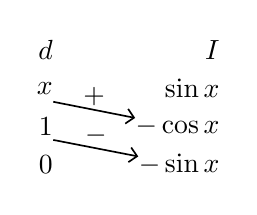
\begin{tikzpicture}[
every edge/.style = {draw, -Straight Barb, semithick, black},
every edge quotes/.append style = {inner sep=1pt, anchor=south},
         M/.style = {matrix of math nodes,
                     nodes = {inner sep=0pt, minimum height=2.2ex, anchor=east},
                     column sep=3em,
                     row sep=1ex}
                    ]

\matrix (m) [M]
{
d & I\\
x & \sin x \\
1 & - \cos x \\
0 & - \sin x \\
};
\draw   (m-2-1.south east) edge ["$+$"]   (m-3-2)
        (m-3-1.south east) edge ["$-$"]   (m-4-2);
\end{tikzpicture}
$$
\begin{align}
&= \frac{\sqrt{2}}{2\pi}(\sin(x)-x\cos(x))\biggr\rvert_{x=-\pi}^\pi\nonumber\\
&= \frac{\sqrt{2}}{2\pi}(\sin(\pi)-\pi\cos(\pi) + \sin(\pi) -\pi\cos(-\pi))\nonumber\\
&= \frac{\sqrt{2}}{2\pi}(2\pi) \implies \int_{-\pi}^\pi x\sin(x)\mathrm{d}x = 2\pi\\
&= \sqrt{2}\nonumber
\end{align}
\begin{align}
\langle x \mid \sqrt{2}\cos(x) \rangle & = \frac{1}{2\pi} \int_{-\pi}^\pi x\sqrt{2}\cos(x)\mathrm{d}x\nonumber\\
&=\frac{\sqrt{2}}{2\pi}\nonumber\int_{-\pi}^\pi x\cos(x)\mathrm{d}x
\end{align}
Similarly, we can use tabular integration to compute this integral.
$$
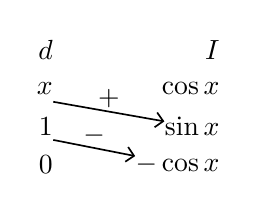
\begin{tikzpicture}[
every edge/.style = {draw, -Straight Barb, semithick, black},
every edge quotes/.append style = {inner sep=1pt, anchor=south},
         M/.style = {matrix of math nodes,
                     nodes = {inner sep=0pt, minimum height=2.2ex, anchor=east},
                     column sep=3em,
                     row sep=1ex}
                    ]

\matrix (m) [M]
{
d & I\\
x & \cos x \\
1 & \sin x \\
0 & - \cos x \\
};
\draw   (m-2-1.south east) edge ["$+$"]   (m-3-2)
        (m-3-1.south east) edge ["$-$"]   (m-4-2);
\end{tikzpicture}
$$
\begin{align}
&=\frac{\sqrt{2}}{2\pi}(x\sin(x)+\cos(x))\biggr\rvert_{x=-\pi}^\pi\nonumber\\
&=\frac{\sqrt{2}}{2\pi}(\pi\sin(\pi)+\cos(\pi)-\pi\sin(-\pi)-\cos(-\pi))\nonumber
\end{align}
\begin{align}
&=\frac{\sqrt{2}}{2\pi}(0)\nonumber\\
&=0\nonumber
\end{align}
Thus $\vec{b}_3=x-\sqrt{2}\sqrt{2}\sin(x)=x-2\sin(x)$. Now we must normalize it by finding its length and dividing by it.
\begin{align*}
\langle x - 2\sin(x) \mid x - 2\sin(x) \rangle & = \frac{1}{2\pi} \int_{-\pi}^\pi (x-2\sin(x))^2 \mathrm{d}x\\
&=\frac{1}{2\pi}\int_{-\pi}^\pi x^2-4x\sin(x)+4\sin^2(x)\mathrm{d}x\\
&=\frac{1}{2\pi}\left(\int_{-\pi}^\pi x^2\mathrm{d}x - 4\int_{-\pi}^\pi x\sin(x)\mathrm{d}x + 4\int_{-\pi}^\pi\sin^2(x)\mathrm{d}x\right)\\
&=\frac{1}{2\pi}\left(\frac{x^3}{3}\biggr\rvert_{x=-\pi}^\pi - 4(2\pi)+4(\pi)\right) \qquad \text{By (1) and (2)}\\
&=\frac{1}{2\pi}\left(\frac{2\pi^3}{3} - 4\pi\right)\\
&=\frac{\pi^2}{3}-2=\frac{\pi^2-6}{3}
\end{align*}
This means that $||\vec{b}_3||=\sqrt{\frac{\pi^2-6}{3}}$, and normalizing our $\vec{b}_3$ we see that our third orthonormal basis vector is $\sqrt{\frac{3}{\pi^2-6}}(x-2\sin(x))$.
\vspace{1em}
\hrule
\vspace{1em}
$$
\vec{b}_4 = x^2-\langle x^2\mid\sqrt{2}\sin(x)\rangle\sqrt{2}\sin(x)-\langle x^2\mid\sqrt{2}\cos(x)\rangle\sqrt{2}\cos(x)-\langle x^2\mid\sqrt{\frac{3}{\pi^2-6}}(x-2\sin(x)\rangle\sqrt{\frac{3}{\pi^2-6}}(x-2\sin(x))
$$
Since $\sqrt{2}\sin(x)$ is odd and $x^2$ is even, their product will be odd. Thus the inner product will evaluate to zero. 
\begin{align}
\langle x^2 \mid\sqrt{2}\cos(x)\rangle &= \frac{1}{2\pi}\int_{-\pi}^\pi x^2\sqrt{2}\cos(x)\mathrm{d}x\nonumber\\
&=\frac{\sqrt{2}}{2\pi} \int_{-\pi}^\pi x^2\cos(x)\mathrm{d}x\nonumber
\end{align}
We can evaluate the integral using tabular integration
$$
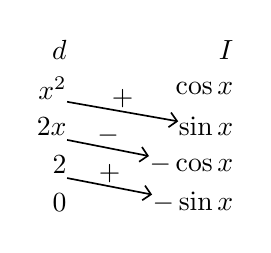
\begin{tikzpicture}[
every edge/.style = {draw, -Straight Barb, semithick, black},
every edge quotes/.append style = {inner sep=1pt, anchor=south},
         M/.style = {matrix of math nodes,
                     nodes = {inner sep=0pt, minimum height=2.2ex, anchor=east},
                     column sep=3em,
                     row sep=1ex}
                    ]

\matrix (m) [M]
{
d & I\\
x^2 & \cos x \\
2x & \sin x \\
2 & -\cos x \\
0 & - \sin x \\
};
\draw   (m-2-1.south east) edge ["$+$"]   (m-3-2)
        (m-3-1.south east) edge ["$-$"]   (m-4-2)
        (m-4-1.south east) edge ["$+$"] (m-5-2);
\end{tikzpicture}
$$
\begin{align}
&=\frac{\sqrt{2}}{2\pi}(x^2\sin(x)+2x\cos(x)-2\sin(x))\biggr\rvert_{x=-\pi}^\pi\nonumber\\
&=\frac{\sqrt{2}}{2\pi}(2\pi\cos(\pi)+2\pi\cos(-\pi))\nonumber\\
&=\frac{\sqrt{2}}{2\pi}(-4\pi)\implies \int_{-\pi}^\pi x^2\cos(x)\mathrm{d}x = -4\pi\\
&=-2\sqrt{2}\nonumber
\end{align}
\begin{align}
\langle x^2 \mid \sqrt{\frac{3}{\pi^2-6}}(x-2\sin(x)) \rangle&=\frac{1}{2\pi} \int_{-\pi}^\pi x^2 \sqrt{\frac{3}{\pi^2-6}}(x-2\sin(x)) \mathrm{d}x\nonumber\\
&=\frac{1}{2\pi}\sqrt{\frac{3}{\pi^2-6}} \int_{-\pi}^\pi x^2(x-2\sin(x))\mathrm{d}x\nonumber\\
&=\frac{1}{2\pi}\sqrt{\frac{3}{\pi^2-6}} \int_{-\pi}^\pi x^3 - 2x^2\sin(x)\mathrm{d}x\nonumber
\end{align}
We saw before that $x^2\sin(x)$ is odd, and $x^3$ is also odd, so the entire function is odd. Since the parity of the function is odd, that means that the integral will evaluate to 0. This means that $\vec{b}_4 = x^2 + 4\cos(x)$, now we must normalize it.
\begin{align}
\langle x^2 + 4\cos(x) \mid x^2 + 4\cos(x) \rangle &= \frac{1}{2\pi} \int_{-\pi}^\pi (x^2+4cos(x))^2\mathrm{d}x\nonumber\\
&= \frac{1}{2\pi} \int_{-\pi}^\pi x^4+8x^2\cos(x)+16\cos^2(x)\mathrm{d}x\nonumber\\
&=  \frac{1}{2\pi}\left(\int_{-\pi}^\pi x^4 \mathrm{d}x + 8\int_{-\pi}^\pi x^2\cos(x)\mathrm{d}x +16\int_{-\pi}^\pi \cos^2(x)\mathrm{d}x\right)\nonumber\\
&= \frac{1}{2\pi}\left(\frac{x^5}{5}\biggr\rvert_{x=-\pi}^{\pi} + 8(-4\pi) + 16(\pi)\right)\qquad\text{By (2) and (4)}\nonumber\\
&= \frac{1}{2\pi}\left(\frac{2\pi^5}{5}-16\pi\right)\nonumber\\
&= \frac{\pi^4}{5}-8 = \frac{\pi^4-40}{5}\nonumber
\end{align}
Thus we can conclude that $||\vec{b}_4||=\sqrt{\frac{\pi^4-40}{5}}$, and after normalizing $\vec{b}_4$ we find the the last orthonormal basis vector is $\sqrt{\frac{5}{\pi^4-40}}(x^3+4\cos(x))$. \\
\\
\noindent Thus we can say that an orthonormal basis for the $\operatorname{span}(\sin(x), \cos(x), x, x^2)$ is 
$$\langle\sqrt{2}\sin(x),\sqrt{2}\cos(x),\sqrt{\frac{3}{\pi^2-6}}(x-2\sin(x)),\sqrt{\frac{5}{\pi^4-40}}(x^3+4\cos(x))\rangle$$

\qs{}{ Let $W \subseteq C([-\pi, \pi])$ be $W=\operatorname{span}\left(\sin (x), \cos (x), x, x^2\right)$. Your answer from problem 4 should be an orthonormal basis for $W$. Compute:\\
(a) $\operatorname{proj}_W(1)$\\
(b) $\operatorname{proj}_W(x \sin (x))$}
\begin{note}
Recall: \\
If $\langle \vec{u}_1, \ldots, \vec{u}_n \rangle$ is an orthonormal basis for $W$, then
$$
\operatorname{proj}_W(\vec{v}) = \sum_{k=1}^n \langle \vec{v} \mid \vec{u}_k \rangle \vec{u}_k
$$
\end{note}
\sol \\
(a)
Using the formula from above, we can begin by computing the inner-products for each summand.
$$
\langle 1 \mid \sqrt{2}\sin(x) \rangle = \frac{1}{2\pi} \int_{-\pi}^\pi \sqrt{2}\sin(x)\mathrm{d}x = 0
$$
This integral evaluates to zero since $\sin(x)$ is odd.
$$
\begin{aligned}
\langle 1 \mid \sqrt{2}\cos(x) \rangle &= \frac{1}{2\pi} \int_{-\pi}^\pi  \sqrt{2}\cos(x)\mathrm{d}x\\
&=\frac{\sqrt{2}}{2\pi} \int_{-\pi}^\pi \cos(x)\mathrm{d}x\\
&=\frac{\sqrt{2}}{2\pi} \sin(x)\biggr\rvert_{x=-\pi}^\pi\\
&=\frac{\sqrt{2}}{2\pi}(0) = 0
\end{aligned}
$$
Since this integral evaluates to zero, then the summand is also nullified, so we will continue.
$$
 \langle 1 \mid \sqrt{\frac{3}{\pi^2-6}}(x-2\sin(x)) \rangle = \frac{1}{2\pi} \int_{-\pi}^\pi \sqrt{\frac{3}{\pi^2-6}}(x-2\sin(x))\mathrm{d}x
$$
Like the first summand that we evaluated, the function is odd, so thus the integral will evaluate to zero.
$$
\begin{aligned}
\langle 1 \mid \sqrt{\frac{5}{\pi^4-40}}(x^3+4\cos(x))\rangle &=  \frac{1}{2\pi} \int_{-\pi}^\pi\sqrt{\frac{5}{\pi^4-40}}(x^3+4\cos(x))\mathrm{d}x\\
&=\frac{1}{2\pi}\sqrt{\frac{5}{\pi^4-40}} \int_{-\pi}^\pi x^3 + 4\cos(x)\mathrm{d}x\\
&=\frac{1}{2\pi}\sqrt{\frac{5}{\pi^4-40}} \left(\int_{-\pi}^\pi x^3\mathrm{d}x + 4\int_{-\pi}^\pi\cos(x)\mathrm{d}x\right)
\end{aligned}
$$
Since $x^3$ is odd, that integral will evaluate to zero, and as we saw in previously the integral of $\cos(x)$ from $x=-\pi$ to $\pi$ evaluates to zero as well. Since all the summands evaluate to zero, then $\operatorname{proj}_W(1) = 0$. \\
\\
\noindent(b) Lets follow the same process as (a), by first evaluating the summands.
$$
\langle x\sin(x) \mid \sqrt{2}\sin(x) \rangle = \frac{1}{2\pi} \int_{-\pi}^\pi x\sin(x)\sqrt{2}\sin(x)\mathrm{d}x = 0
$$
This evaluates to zero since we're multiplying an even function by an odd function. Thus the first summand will be nullified and is not necessary for the projection of $x\sin(x)$.
$$
\begin{aligned}
\langle x\sin(x) \mid \sqrt{2}\cos(x) \rangle &= \frac{1}{2\pi} \int_{-\pi}^\pi x\sin(x)\sqrt{2}\cos(x)\mathrm{d}x\\
&= \frac{\sqrt{2}}{2\pi} \int_{-\pi}^\pi x\sin(x)\cos(x)\mathrm{d}x\\
&= \frac{\sqrt{2}}{2\pi} \int_{-\pi}^\pi \frac{x\sin(2x)}{2}\mathrm{d}x\qquad\text{By double angle formula}\\
&= \frac{\sqrt{2}}{4\pi} \int_{-\pi}^\pi x\sin(2x)\mathrm{d}x
\end{aligned}
$$
We can use tabular integration to complete this integral
$$
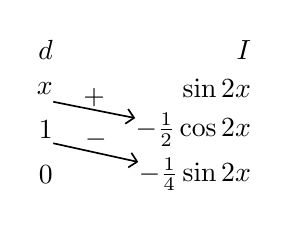
\begin{tikzpicture}[
every edge/.style = {draw, -Straight Barb, semithick, black},
every edge quotes/.append style = {inner sep=1pt, anchor=south},
         M/.style = {matrix of math nodes,
                     nodes = {inner sep=0pt, minimum height=2.2ex, anchor=east},
                     column sep=3em,
                     row sep=1ex}
                    ]

\matrix (m) [M]
{
d & I\\
x & \sin 2x \\
1 & -\frac{1}{2}\cos 2x\\
0 & -\frac{1}{4}\sin 2x \\
};
\draw   (m-2-1.south east) edge ["$+$"]   (m-3-2)
        (m-3-1.south east) edge ["$-$"]   (m-4-2);
\end{tikzpicture}
$$
$$
\begin{aligned}
&=\frac{\sqrt{2}}{4\pi}\left(\frac{1}{4}\sin(2x)-\frac{1}{2}x\cos(2x)\right)\biggr\rvert_{x=-\pi}^\pi\\
&=\frac{\sqrt{2}}{8\pi}\left(-\pi\cos(2\pi)-\pi\cos(-2\pi)\right) = -\frac{\sqrt{2}}{4}
\end{aligned}
$$
$$
\langle x\sin(x) \mid \sqrt{\frac{3}{\pi^2-6}}(x-2\sin(x)) \rangle =\frac{1}{2\pi} \int_{-\pi}^\pi x\sin(x)\sqrt{\frac{3}{\pi^2-6}}(x-2\sin(x))\mathrm{d}x = 0
$$
This inner-product evaluates to zero since we multiply an even function by an odd function. Thus this summand will be nullified and is not necessary for the projection of $x\sin(x)$.
$$
\begin{aligned}
\langle x\sin(x) \mid \sqrt{\frac{5}{\pi^4-40}}(x^3+4\cos(x)) \rangle &= \frac{1}{2\pi} \int_{-\pi}^\pi x\sin(x)\sqrt{\frac{5}{\pi^4-40}}(x^3+4\cos(x))\mathrm{d}x\\
&=\frac{1}{2\pi}\sqrt{\frac{5}{\pi^4-40}}\int_{-\pi}^\pi x\sin(x)(x^3+4\cos(x))\mathrm{d}x\\
&=\frac{1}{2\pi}\sqrt{\frac{5}{\pi^4-40}}\left(\int_{-\pi}^\pi x^4\sin(x)\mathrm{d}x + 4 \int_{-\pi}^\pi x\cos(x)\sin(x)\mathrm{d}x\right)\\
&=\frac{1}{2\pi}\sqrt{\frac{5}{\pi^4-40}}(0 + -2\pi)\\
&=-\sqrt{\frac{5}{\pi^4-40}}
\end{aligned} 
$$
Since we have computed all the inner-products, we can now find the projection of $x\sin(x)$.
$$
\begin{aligned}
\operatorname{proj}_W(x\sin(x)) &= -\frac{\sqrt{2}}{4}\sqrt{2}\cos(x) - \sqrt{\frac{5}{\pi^4-40}}^2(x^3+4\cos(x))\\
&=-\frac{1}{2}\cos(x) - \frac{5x^3 + 20\cos(x)}{\pi^4-40}
\end{aligned}
$$ 
\qs{}{ Let $A$ be as in problem 3.\\
(a) Compute the matrix of $\operatorname{proj}_{\operatorname{ran}(A)}$, that is, find the matrix $M$ so that $M \vec{x}=\operatorname{proj}_{\operatorname{ran}(A)}(\vec{x})$ for all $\vec{x} \in \mathbb{R}^3$.\\
(b) For each of the following $\vec{b}_i$ compute $\operatorname{proj}_{\operatorname{ran}(A)}\left(\vec{b}_i\right)$ :
$$
\vec{b}_1=\left[\begin{array}{l}
2 \\
1 \\
2
\end{array}\right] \quad \vec{b}_2=\left[\begin{array}{l}
1 \\
2 \\
3
\end{array}\right] \quad \vec{b}_3=\left[\begin{array}{l}
1 \\
1 \\
1
\end{array}\right] \quad \vec{b}_4=\left[\begin{array}{l}
3 \\
2 \\
2
\end{array}\right]
$$
(c) For each $\vec{b}_i$ from (b), let $\hat{b}_i=\operatorname{proj}_{\operatorname{ran}(A)}\left(\vec{b}_i\right)$, each $\hat{b}_i$ has $\hat{b}_i \in \operatorname{ran}(A)$ and so there is a solution to
$$
A \hat{x}=\hat{b}_i .
$$

Use $\operatorname{ker}(A)$ and the change of basis matrix you found in problem 3 to find full solution sets to
$$
A \hat{x}_i=\hat{b}_i
$$
for each $i=1,2,3,4$.}
\begin{note}
Recall: \\
If $W \subseteq \mathbb{R}^n$, there exists a matrix for $\operatorname{proj}_W$. If $\langle \vec{u}_1, \ldots, \vec{u}_n \rangle$ is an orthonormal basis for $W$ then let
$$
Q = \begin{bmatrix} 
\vline&\vline&&\vline\\
\vec{u}_1&\vec{u}_2&\ldots&\vec{u}_n\\
\vline&\vline&&\vline\\
\end{bmatrix}
$$
Then $\operatorname{proj}_W(\vec{x}) = QQ^\top\vec{x}$
\end{note}
\sol \\
(a)
$$
Q = \begin{bmatrix}
1/\sqrt{5}&4\sqrt{5}/15\\
0&\sqrt{5}/3\\
2/\sqrt{5}&-2\sqrt{5}/15
\end{bmatrix} \qquad \qquad
Q^\top = \begin{bmatrix}
1/\sqrt{5}&0&2\sqrt{5}\\
4\sqrt{5}/15&\sqrt{5}/3&-2\sqrt{5}/15
\end{bmatrix}
$$
$$
QQ^\top =
\begin{bmatrix}
5/9&4/9&2/9\\
4/9&5/9&-2/9\\
2/9&-2/9&8/9
\end{bmatrix}
$$
(b) For each $\vec{b}_i$,  we can apply the formula from my note.
$$
\operatorname{proj}_W(\vec{b}_1) = QQ^\top\vec{b}_1 = \begin{bmatrix}
5/9&4/9&2/9\\
4/9&5/9&-2/9\\
2/9&-2/9&8/9
\end{bmatrix}\begin{bmatrix} 2\\1\\2\end{bmatrix} = \begin{bmatrix}2\\1\\2\end{bmatrix}
$$
\vspace{0.5em}
\hrule
\vspace{1em}
$$
\operatorname{proj}_W(\vec{b}_2) = QQ^\top\vec{b}_2 = \begin{bmatrix}
5/9&4/9&2/9\\
4/9&5/9&-2/9\\
2/9&-2/9&8/9
\end{bmatrix}\begin{bmatrix}1\\2\\3\end{bmatrix} = \begin{bmatrix}19/9\\8/9\\22/9\end{bmatrix}
$$
\vspace{0.5em}
\hrule
\vspace{1em}
$$
\operatorname{proj}_W(\vec{b}_3) = QQ^\top\vec{b}_3 = \begin{bmatrix}
5/9&4/9&2/9\\
4/9&5/9&-2/9\\
2/9&-2/9&8/9
\end{bmatrix}\begin{bmatrix}1\\1\\1\end{bmatrix} = \begin{bmatrix}11/9\\7/9\\8/9\end{bmatrix}
$$
\vspace{0.5em}
\hrule
\vspace{1em}
$$
\operatorname{proj}_W(\vec{b}_4) = QQ^\top\vec{b}_4 = \begin{bmatrix}
5/9&4/9&2/9\\
4/9&5/9&-2/9\\
2/9&-2/9&8/9
\end{bmatrix}\begin{bmatrix}3\\2\\2\end{bmatrix} = \begin{bmatrix}3\\2\\2\end{bmatrix}
$$
(c) We can use the change of basis matrix we found in problem 3 to find solutions to each $\hat{b}_i$.
$$
\vec{x} = P_{\mathfrak{E}\rightarrow\mathfrak{B}}\hat{b}_i
$$
And then use our basis for $ker(A)$ to construct full solution sets.
\vspace{1em}
\hrule
\vspace{1em}
$$
\vec{x} = P_{\mathfrak{E}\rightarrow\mathfrak{B}}\hat{b}_1 = \begin{bmatrix}-2&2&1\\1&-2&0\\0&1&0\end{bmatrix}\begin{bmatrix}2\\1\\2\end{bmatrix} = \begin{bmatrix}0\\0\\1\end{bmatrix}
$$
$$
\left\{
\begin{bmatrix}0\\0\\1\end{bmatrix} + c_1\begin{bmatrix}-1\\-1\\1\end{bmatrix} : c_1 \in \mathbb{R}
\right\}
$$
\vspace{0.5em}
\hrule
\vspace{1em}
$$
\vec{x} = P_{\mathfrak{E}\rightarrow\mathfrak{B}}\hat{b}_2 = \begin{bmatrix}-2&2&1\\1&-2&0\\0&1&0\end{bmatrix}
\begin{bmatrix}19/9\\8/9\\22/9\end{bmatrix} = \begin{bmatrix}0\\1/3\\8/9\end{bmatrix}
$$
$$
\left\{
\begin{bmatrix}0\\1/3\\8/9\end{bmatrix} + c_1\begin{bmatrix}-1\\-1\\1\end{bmatrix} : c_1 \in \mathbb{R}
\right\}
$$
\vspace{0.5em}
\hrule
\vspace{1em}
$$
\vec{x} = P_{\mathfrak{E}\rightarrow\mathfrak{B}}\hat{b}_3 = \begin{bmatrix}-2&2&1\\1&-2&0\\0&1&0\end{bmatrix}
\begin{bmatrix}11/9\\7/9\\8/9\end{bmatrix} = \begin{bmatrix}0\\-1/3\\7/9\end{bmatrix}
$$
$$
\left\{
 \begin{bmatrix}0\\-1/3\\7/9\end{bmatrix}+ c_1\begin{bmatrix}-1\\-1\\1\end{bmatrix} : c_1 \in \mathbb{R}
\right\}
$$
\vspace{0.5em}
\hrule
\vspace{1em}
$$
\vec{x} = P_{\mathfrak{E}\rightarrow\mathfrak{B}}\hat{b}_3 = \begin{bmatrix}-2&2&1\\1&-2&0\\0&1&0\end{bmatrix}\begin{bmatrix}3\\2\\2\end{bmatrix} = \begin{bmatrix}0\\-1\\2\end{bmatrix}
$$
$$
\left\{
\begin{bmatrix}0\\-1\\2\end{bmatrix}+ c_1\begin{bmatrix}-1\\-1\\1\end{bmatrix} : c_1 \in \mathbb{R}
\right\}
$$
\end{document}

